
\section{Introduction and Motivation}

Exploring long term alternatives to the CMOS technology is gaining
more and more revelance as the scaling trend of such devices keeps
introducing new challenges. Power density, defect tolerance, testing
costs and wire delays are only a few of the many critical aspects
involved~\cite{}. While software parallelism and multicore
approaches~\cite{TODO} are partially mitigating the impact of such
constraints on performances, it is likely that the growing computing demand will
eventually need even more radical architectural modifications and new
paradigms in order to address the Computer Design challenges of the next
decades.

In the last years, Self-assembled nanoscale architectures~\cite{TOOD}
are emerging as a promising technology due their tera/peta scale of
integration, defect tolerance tolerance and huge potential computing
capabilities~\cite{TODO}. These technologies are certainly still at
their early stage of development, however different laboratory demos and
prof-of-concepts architectures have been presented~\cite{TODO}.
The main idea behind this approach is to exploit the physical regularity and
stabiliy of DNA structures in order to create a scaffold onto which
nano-devices (e.g. nanowires and nanotubes~\cite{TODO}) can be
attached. This can be achieved by designing approapriate complementary DNA tags for
each terminal to be placed, so that a nano device will be attached
only where its own DNA tag matches a complementary tag on the DNA grid
scaffold (see figure~\ref{fig:dna_tag}.
\begin{figure}
  \centering
    \includegraphics[width=0.40\textwidth]{pictures/dna_tag.ps}
  \caption{DNA tag matching}
  \label{fig:dna_tag}
\end{figure}
A detailed description of the chemical properties involved is far
beyond the scope of this paper (see also~\cite{}), so we will focus on
the three main challenges that this new fabrication process introduces
in Computer Design: (i)limited node complexity, (ii) large scale
randomness and (iii) high defect rates.  

The \emph{limited node complexity} aspect is directly
related to the use of complementary DNA tags in order to place circuit
components. In a traditional CMOS process the complexity is introduced
using a photolithography mask, so that larger (more complex) circuits
only require larger masks; conversely, self-assembly achieves
complexity by increasing the number of unique DNA tags, since more
different tags means having more control on component placement. Ideally, by specifying a single
and unique tag for each nano transistor terminal, we could exactly
choose where each component would be placed. But the number of DNA
symbols forming the DNA sequence is limited (sequence of 4 nucleobases
G,A,T,C) and so creating many different tags (of a given lenght) would
mean make them more similar to each other, increasing the probability
of incorrect/partial matching. To avoid this problem we should limit
the number of unique tags, thus limiting the complexity at each node. 

\emph{Large scale randomness} and \emph{high defect rates} are the other two fundaments
conditions of self-assembled technology: if, as seen, some complexity
can be introduced by designing tag sequences in the DNA grid of each
node, we have no control of where each of these grids will be placed
on the whole network. Further, as a consequence, we cannot guarantee
other typical properties of regular networks, like nodes being
connected to 4 neighbors, having a determined orientation and so on.

These aspects of a DNA-self assembly process lead to some important
architectural implications to be addressed when approaching to the
Computer Design: computational model must be founded on a distributed
network of small computing and storage nodes, randomly placed and
interconnected (see figure~\ref{fig:nana}).  Proof-of-concept of such kind of computational model
can be found in~\cite{}, where instructions and data operands travel
on packets and routed using a topology-agnostic strategy that avoids
deadlock, since no particular regularity can be assumed in such
network. Altought we will assume a similar scenario as background, it
is important to underline that the proposed approach to defect
tolerance is more general and not stricly dependent on any of these
architectures.
\begin{figure}
  \centering
    \includegraphics[width=0.40\textwidth]{pictures/nana.ps}
  \caption{Irregular architecture of computing and storage elements}
  \label{fig:nana}
\end{figure}

Several works~\cite{} have been presented addressing the problem of topology
agnostic routing. While they show interesting
performances, the requirement for virtual channels resources 
to avoid deadlock makes them not suitable for the specific DNA self
assembled networks we are assuming as background.
Other topology independent algorithms~\cite{} don't use virtual channels to
achieve deadlock freedom, but turn proibitions. However,
the centralized nature of these algorithms still makes it necessary to
provide a topology graph as input to generate a working set
of proibitions and routing tables.
Up-Down~\cite{} exploits the creation of a spanning tree of the
topology, then placing bidirectional restrictions by avoiding a packet
to traverse the same link in both up and down directions.
While the hierarchical nature of this approach can lead to uneven traffic
distribution, with many packets traversing upper links (near to the
root), this is quite acceptable in classical wide area networks
topologies with a limited number of nodes. Other approaches~\cite{} mitigate this
issue, but the set of turn restrictions is still prefixed,
striclty depending on the particular tree root selected, thus making these
approaches not scalable for the TODO(thousands) nodes scenario of DNA
self assembled technology.

Other solutions~\cite{} try to approach the issue of irregular
topologies by limiting the number and location of missing links. This
restriction is clearly unacceptable given the hight-defect rates of
DNA self-assembled networks scenario. For the same reason, we also
avoid considering solutions based on hardware-redundancy to
dynamically recover defects as in~\cite{}. 

In~\cite{} authors present SR, an approach the solves these
limitations by allowing turn restrictions to be placed locally,
independently from other restrictions. The whole network is
partitioned into segments, and a each bidirectional turn
restriction can be freely chosen within a segment in order to guarantee
deadlock freedom and connected networks. This \emph{locality
independence} property, together with no requirement of any particular tree/root
choice, would make it the best choice for the given scenario;
however, its topology independency still requires the knowledge of the
whole network graph in order to find the segments. 

The contribution presented in this paper is a first effort for a
Distributed Segment-based routing in nanoscale DNA based networks
(DiSR). Given the particular scenario assumed as background, is essential
avoiding non-scalable or resource hungry solutions such as
centralized node algorithms, tree-based approaches, virtual channels
or other expensive hardware implementations. While maintaining similar
properties to segment-based routing, the DiSR approach is not intended
to discover the "optimal" segment choice (ideally reachable with the
knowledge of the topology graph) but just to demonstrate a concrete
model that can fit into such complex, irregular and large sized
topologies.

The paper is organized as follows: in Section~\ref{sec:disr_concepts}
we introduce the main elements of the DiSR approach, describing  
a draft of the DiSR model in Section~\ref{sec:disr_model}
together with execution model details in Section~\ref{sec:disr_detaled_model}.
Finally, simulations are carried out with the opensource tool Nanoxim
to demostrate how DiSR preserves some of the main segment-based
properties and how compares to the tree-based approaches.


